\documentclass[../TDM3_courbe_app.tex]{subfiles}%

\begin{document}
\section[s]"2"{Oscillations d'un anneau sur un cerceau}
\noindent
\begin{minipage}[c]{.74\linewidth}
	\enonce{%
		Un cerceau de centre O et de rayon $R$ est maintenu dans un plan vertical,
		et un anneau de masse $m$ assimilé à un point matériel M peut glisser sans
		frottements le long de ce cerceau.
	}
	\QR{%
		Qu'est-ce que l'hypothèse «~sans frottements~» implique pour la
		réaction du cerceau sur l'anneau~?
	}{%
		L'hypothèse «~sans frottements~» signifie que la réaction du cerceau
		est uniquement normale~: il n'y a pas de composante tangentielle.
	}
\end{minipage}
\begin{minipage}[c]{.25\linewidth}
	~
	\begin{center}
		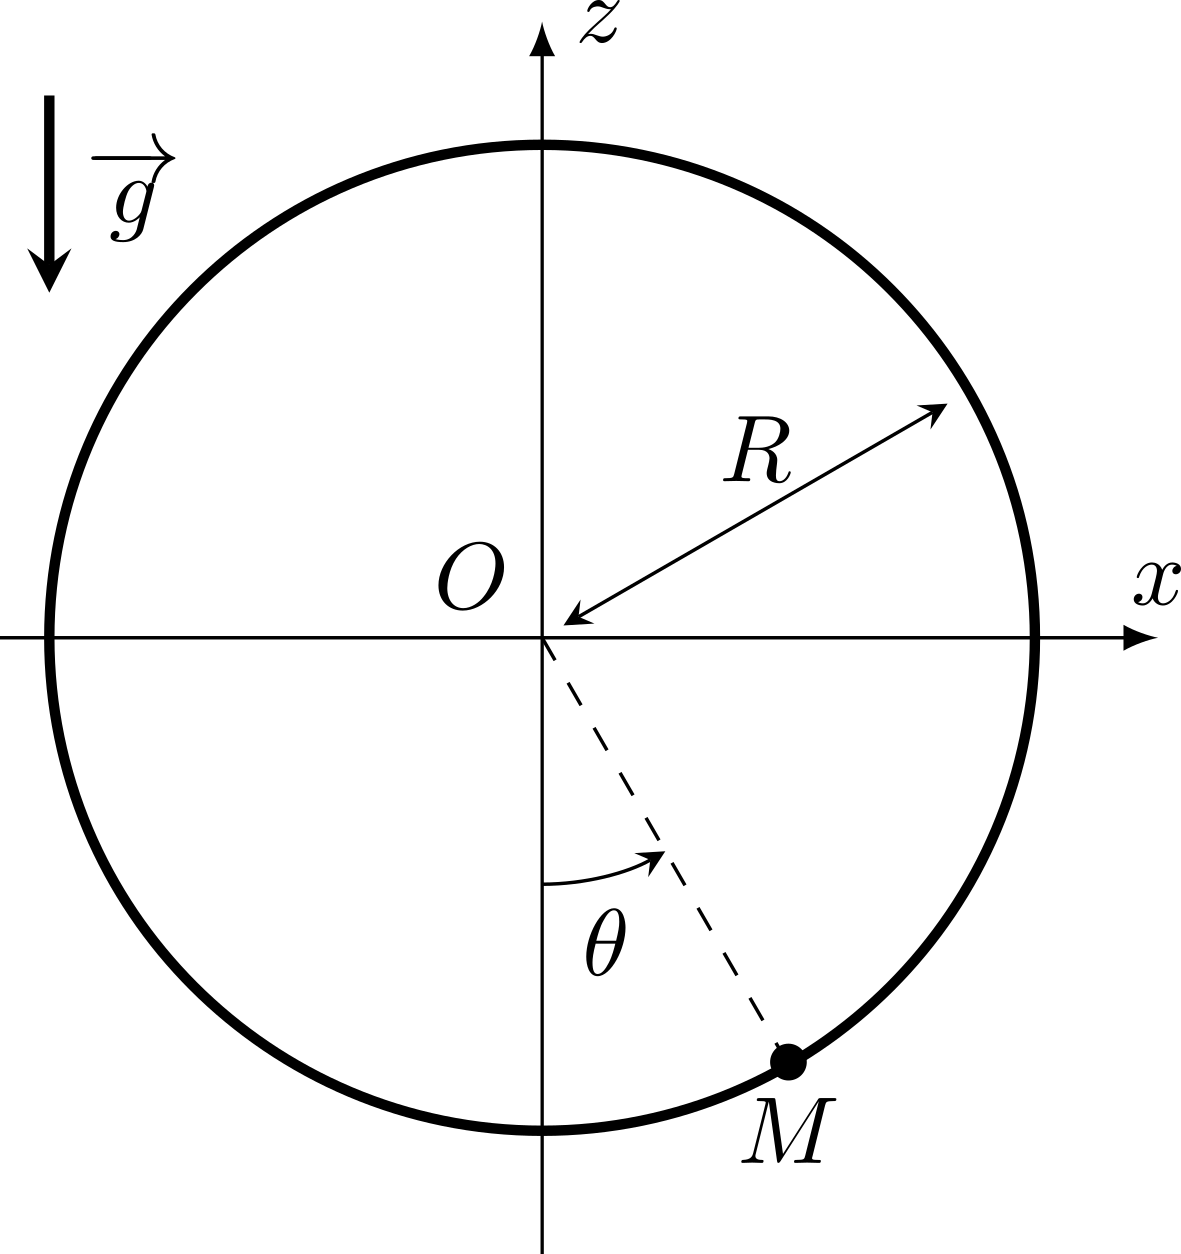
\includegraphics[width=\linewidth]{anneau_cerceau-plain}
	\end{center}
\end{minipage}

\QR<[start=2]>{%
	Écrire le PFD appliqué à l'anneau et le projeter dans une base
	adaptée.
}{%
	\begin{itemize}
		\item[b]{Système}~: \{anneau\}
		\item[b]{Référentiel}~: $\Rc\ind{sol}$ supposé galiléen
		\item[b]{Repère}~: $(\Or,\ur,\ut)$ avec $\ut$ dans le sens de $\th$
		\item[b]{Repérage}~:
		\begin{align*}
			\OM(t) & = R\ur                 \\
			\vf(t) & = R\tp\ut              \\
			\af(t) & = R\tpp\ut - R\tp^2\ur
		\end{align*}
		\item[b]{BDF}~:
		\[
			\begin{array}{ll}
				\textbf{Poids}    & \Pf = mg(\cos\th\ur -\sin\th\ut) \\
				\textbf{Réaction} & \Rf = -R_N\ur
			\end{array}
		\]
		\item \leftcenters{\textbf{PFD}~:}{
			      $\DS
				      m\af = \Pf + \Rf
				      \Lra
				      \mqty(-mR\tp^2\\mR\tpp) = \mqty(mg\cos\th-R_N\\-mg\sin\th)
			      $}
		      \begin{empheq}[box=\fbox, left=\Lra\empheqlbrace]{align}
			      mg\cos\th + mR\tp^2 & = R_N\notag\\
			      \label{eq:pendb}
			      mR\tpp + mg\sin\th & = 0
		      \end{empheq}
	\end{itemize}
}
\QR{%
	En déduire l'équation différentielle régissant le mouvement.
}{%
	Avec \eqref{eq:pendb}, en la mettant sous forme canonique~:
	\begin{equation}\label{eq:pendc}
		\tpp + \frac{g}{R}\sin\th = 0
		\Lra
		\boxed{\tpp + \w_0{}^2\sin\th = 0}
	\end{equation}
	\leftcenters{\hspace{-10pt}avec}{$\DS\boxed{\w_0 = \sqrt{\frac{g}{R}}}$}
}
\enonce{%
	On se place dans l'approximation des petits angles ($\abs{\th} < \th_0 =
		\ang{20}$). Initialement, l'anneau est situé à la verticale en-dessous de O et
	il est lancé vers la droite, avec une vitesse initiale de norme $v_0$.
}
\QR{%
	En déduire l'équation horaire du mouvement.
}{%
	On a donc
	\[
		\boxed{\th(0) = 0}
		\qet
		\vf(0) = v_0\ut = R\tp(0)\ut
		\Lra
		\boxed{\tp(0) = \frac{v_0}{R}}
	\]
	L'équation~\eqref{eq:pendc} se simplifie avec $\sin\th\approx\th$, pour
	donner
	\begin{gather*}
		\boxed{\tpp + \w_0{}^2\th = 0}
		\\\Ra
		\th(t) = A\cos(\w_0t) + B\sin(\w_0t)
		\shortintertext{Et avec les CI,}
		\th(0) = 0
		\Lra
		\boxed{A = 0}
		\\
		\tp(0) = \frac{v_0}{R}
		\Lra
		\boxed{B = \frac{v_0}{R\w_0}}
		\\\Ra
		\boxed{
			\th(t) = \frac{v_0}{R\w_0}\sin(\w_0t)}
	\end{gather*}
}
\QR{%
	À quelle condition sur $v_0$ l'approximation des petits angles
	est-elle vérifiée~?
}{%
	La valeur maximale de $\abs{\th(t)}$ est $v_0/(R\w_0)$, quand le
	sinus vaut $\pm1$. Pour avoir des petits angles, il faut que l'angle
	maximal ne dépasse pas $\th_0$, soit
	\begin{gather*}
		\frac{v_0}{R\w_0} < \th_0
		\Lra
		v_0 < \th_0 R \sqrt{\frac{g}{R}}
		\\\Lra
		\boxed{v_0 < \th_0 \sqrt{Rg}}
	\end{gather*}
}

\end{document}
